\documentclass[12pt]{beamer}
%\documentclass[20pt,handout]{beamer}
\usetheme{Darmstadt}
\usepackage{graphicx}
%\usepackage[german]{babel}
\usepackage{ngerman}
\usepackage[T1]{fontenc}
\usepackage[utf8]{inputenc}
\usepackage{tikz}
\setbeamertemplate{footline}[frame number]

\newcommand{\cc}[1]{\includegraphics[height=4mm]{img/#1.png}\hspace{1mm}}
\usepackage{ifthen}
\newcommand{\license}[2][]{\\#2\ifthenelse{\equal{#1}{}}{}{\\\scriptsize\url{#1}}}
\usepackage{textcomp}
\usepackage{hyperref}

\pgfdeclareimage[height=.6cm]{c3d2logo}{./img/c3d2.pdf} 


\pgfdeclarelayer{foreground}
\pgfsetlayers{main,foreground}
\logo{\pgfputat{\pgfxy(-1,0)}{\pgfbox[center,base]{\pgfuseimage{c3d2logo}}}}


\title{Freie Software}
\author{\small Martin Byrenheid, Marius Melzer\\\large Chaos Computer Club Dresden}
\date{11.07.2014}

\begin{document}
\maketitle

\section{CCC}
\subsection{}

\begin{frame}
  \frametitle{Chaos Computer Club}
  \begin{figure}
    
\includegraphics[height=0.7\textheight]{img/fingerabdruck.jpg}
  \end{figure}
\end{frame}

\begin{frame}
  \frametitle{Chaos Computer Club}
  \begin{figure}
    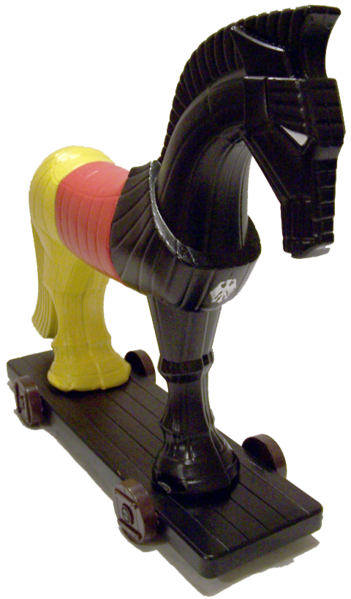
\includegraphics[height=0.7\textheight]{img/trojaner.png}
  \end{figure}
\end{frame}

\begin{frame}
    \frametitle{Chaos Computer Club}
    \begin{itemize}
      \item<1-> Chaos Computer Club Dresden (\url{http://c3d2.de})
          \note{}
      \item<2-> Datenspuren: 13./14.09.2014 \url{http://datenspuren.de}
      \item<3-> Podcasts (\url{http://pentamedia.de})
      \item<4-> Chaos macht Schule
    \end{itemize}
\end{frame}

\section{Probleme}
\subsection{}

\section{Freie Software}


\subsection{GNU 1}
\begin{frame}{Das GNU Projekt}

\begin{columns}


\column{6cm}
\begin{itemize}
\item Begonnen von Richard Stallman im Jahr 1984 
\item Gründung der Free Software Foundation im Jahr 1985 
\end{itemize}

\column{7cm}


\begin{center}
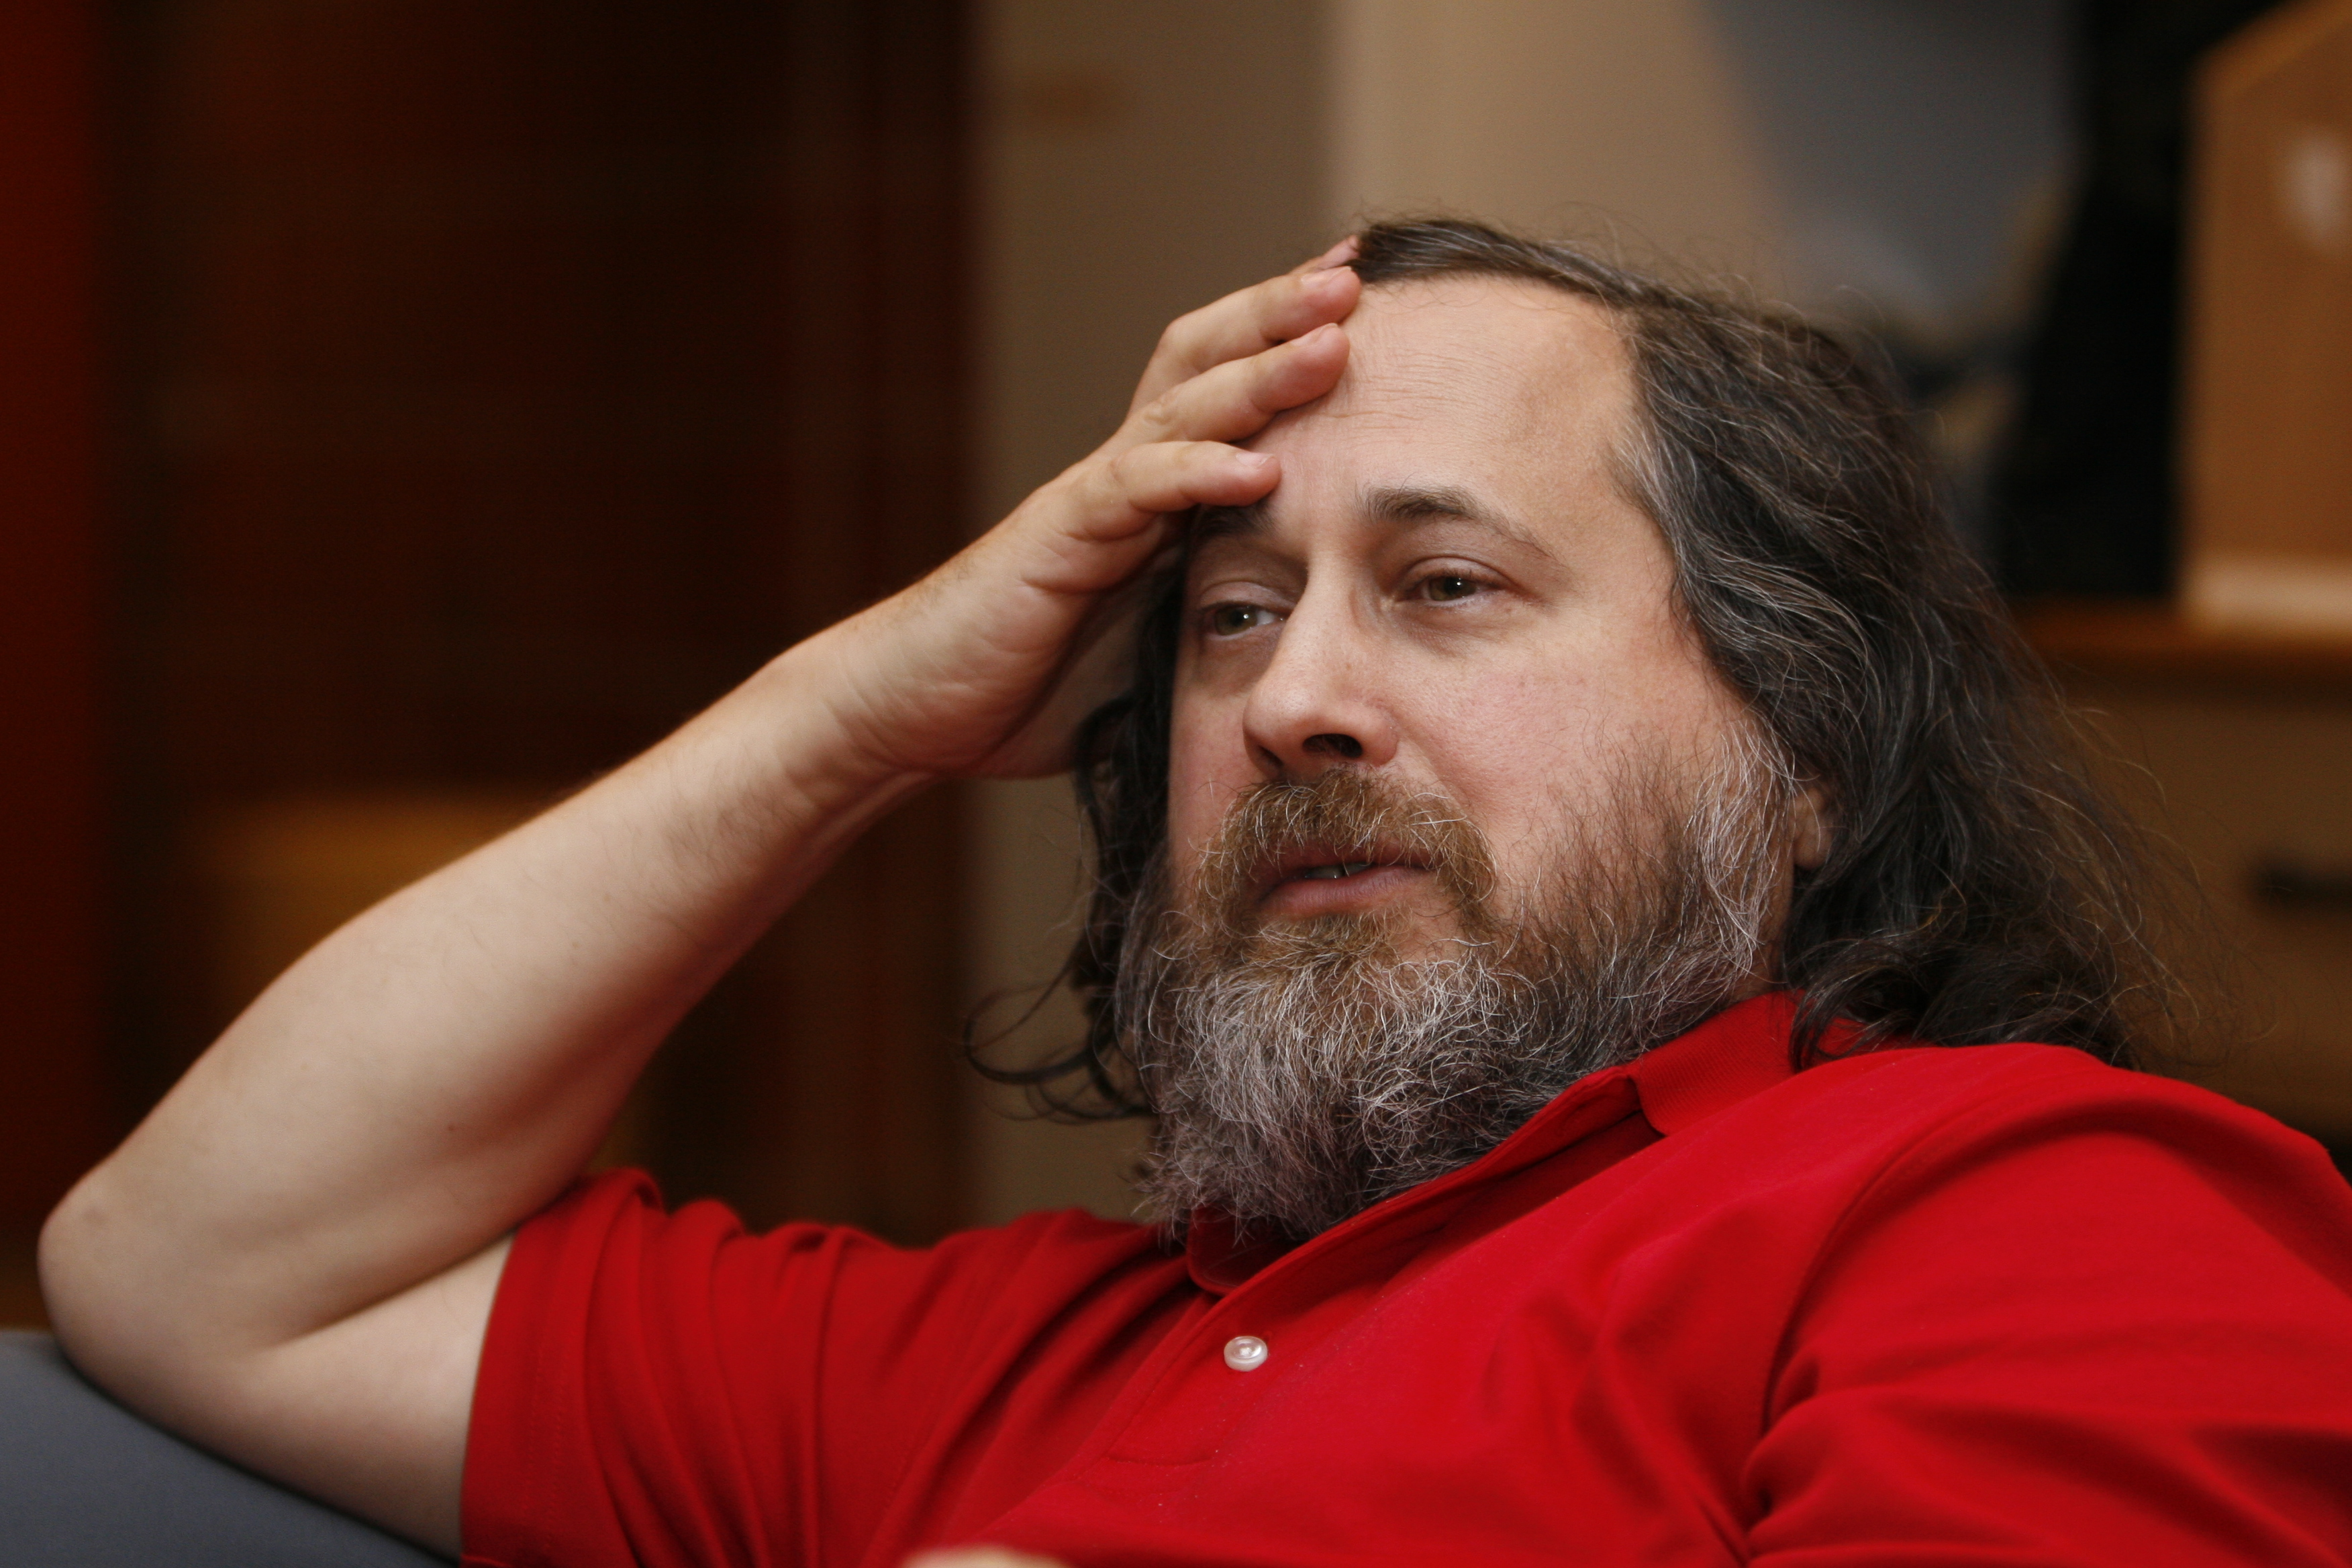
\includegraphics[width=4.5cm]{img/stallman}
\par\end{center}


\begin{center}

\includegraphics[width=5cm]{img/logo-fsf}
\par\end{center}

\end{columns}
\end{frame}



\subsection{GNU 2}
\begin{frame}{Das GNU Projekt}

\begin{itemize}
\item Bekannte Softwarepakete: Emacs, GCC, GPG 
\item Seit 1992 zusammen mit Linux ein komplett freies Betriebssystem \end{itemize}
\begin{quote}
\textquotedbl{}The term “free software” is sometimes misunderstood—it
has nothing to do with price. 

It is about freedom.\textquotedbl{} 
\end{quote}
\end{frame}



\subsection{Freie Software 1}
\begin{frame}{Freie Software}


\textbf{Lizenz} räumt \textbf{vier wesentliche Freiheiten} ein:
\begin{enumerate}
\item[0] Die Freiheit, das Programm auszuführen wie man möchte und für jeden
Zweck.
\item[1] Die Freiheit, die Funktionsweise des Programms zu untersuchen und
eigenen Bedürfnissen der Datenverarbeitung anzupassen.
\item[2] Die Freiheit, das Programm weiter zu verbreiten und damit seinen
Mitmenschen zu helfen.
\item[3] Die Freiheit, das Programm zu verbessern und diese Verbesserungen
der Öffentlichkeit freizugeben, damit die gesamte Gemeinschaft davon
profitiert.
\end{enumerate}
\end{frame}



\subsection{Freie Software 2}
\begin{frame}{Freiheit 0 - Freiheit der Ausführung}


Erlaubt Ausführung
\begin{itemize}
\item auf \textbf{beliebigem Rechner} und
\item für \textbf{beliebige Zwecke}
\end{itemize}

$\rightarrow$ keine vorherige Erlaubnis durch Entwickler oder Unternehmen
erforderlich 

\end{frame}



\subsection{Freie Software 3}
\begin{frame}{Freiheit 1 - Freiheit der Anpassung}

\begin{itemize}
\item Zugang zum Quellcode erforderlich
\item umfasst Freiheit, modifizierte Version statt Original auszuführen
\item besonders relevant für Sicherheits-Aspekte
\end{itemize}
\end{frame}



\subsection{Freie Software 4}
\begin{frame}{Freiheit 2 - Freiheit der Weitergabe}


Kopien können an jedermann überall weitergegeben werden
\begin{itemize}
\item mit oder ohne Modifikation
\item kostenlos oder gegen Vertriebsgebühr
\item keine vorherige Erlaubnis durch durch Entwickler/Unternehmen erforderlich
\end{itemize}
\end{frame}



\subsection{Freie Software 5}
\begin{frame}{Freiheit 3 - Freiheit der Veröffentlichung}

\begin{itemize}
\item eigene Version darf Veröffentlicht werden
\item \textbf{Copyleft-Konzept}

\begin{itemize}
\item erzwingt Freiheit modifizierter/erweiterter Softwareversionen
\item verhindert Umwandlung in proprietäre Software
\item verhindert nachträgliche Änderungen an der Lizenz
\item Umsetzung durch \emph{GNU General Public License}
\end{itemize}
\end{itemize}
\end{frame}



\subsection{Freie Software 6}
\begin{frame}{Freie Software und Open Source}


\textbf{Open Source}
\begin{itemize}
\item offenes Entwicklungsmodell im Vordergrund
\item mehr als nur Offenlegung des Quellcodes (Weiterverwendung, Modifikationen,
Diskriminierung)
\item Lizenzen teilweise restriktiver als freie Lizenzen
\item allgemein große Überlappung zu freier Software
\end{itemize}
\end{frame}

\section{Beispiele für Freie Software}


\subsection{LibreOffice}
\begin{frame}{LibreOffice}

\begin{columns}


\column{6cm}
\begin{itemize}
\item Textverarbeitung
\item Tabellenkalkulation
\item Präsentationen
\item Formeleditor
\item nutzt Open Document Format zur Speicherung
\end{itemize}

\column{5cm}


\begin{center}

\includegraphics[width=5cm]{img/LibreOffice}
\par\end{center}

\end{columns}
\end{frame}



\subsection{Android}
\begin{frame}{Freie Software für Android}

\begin{columns}


\column{6cm}


\textbf{F-Droid}
\begin{itemize}
\item Installationsdienst für freie Android-Software
\end{itemize}

\vspace{0.5cm}



\textbf{TextSecure}
\begin{itemize}
\item Verschlüsselter Nachrichtenaustausch
\item Verschlüsselte Speicherung
\end{itemize}

\column{5cm}


\begin{center}

\includegraphics[width=2cm]{img/F-Droid_Logo_2}
\par\end{center}


\begin{center}

\includegraphics[width=2cm]{img/TextSecure_Icon}
\par\end{center}

\end{columns}
\end{frame}



\subsection{Replicant}
\begin{frame}{Replicant}

\begin{columns}


\column{6cm}
\begin{itemize}
\item basiert auf Android
\item Ziel, alle proprietären Komponenten durch freie zu ersetzen
\item Einbindung von F-Droid
\item \textbf{Problem:} Verlust der Garantie bei Installation
\end{itemize}

\column{5cm}


\begin{center}

\includegraphics[width=2cm]{img/Replicant_logo_alpha}
\par\end{center}

\end{columns}
\end{frame}



\subsection{Linux}
\begin{frame}{Linux}

\begin{columns}


\column{8cm}
\begin{itemize}
\item Weit verbreitet als Server-Betriebssystem
\item Bekannte Desktop-Varianten: 

\begin{itemize}
\item Ubuntu/Debian Linux
\item OpenSUSE
\end{itemize}
\item Können als Live-System ausprobiert werden
\item Integrierte Software für Verschlüsselung, Webbrowsing, E-Mail, Textverarbeitung
etc.
\end{itemize}

\column{6cm}


\begin{center}

\includegraphics[width=3cm]{img/Tux}
\par\end{center}

\end{columns}
\end{frame}

\end{document}
